Die Abschirmungszahl kann durch Umstellen von Formel \eqref{Abschirm} zu
\begin{align}
	\sigma_2 = z - \sqrt[4]{\frac{\Delta E_\text{D}}{R_\infty\alpha^2}l(l+1)n^3} \ ,
\end{align}
direkt berechnet werden. Nachfolgend werden die dafür nötigen Größen aus den Messwerten bestimmt.
\subsection{Umrechnung der gemessenen Winkel}
Als Winkel der Totalreflexion wird
\begin{align}
	\delta = \SI{338.4}{\degree}
\end{align}
gemessen. Mit der Winkelbeziehung \eqref{Beta} kann der Winkel
\begin{align}
	\beta = \SI{59.2}{\degree}
\end{align}
bestimmt werden. Die mit Beziehung \eqref{Beugungswinkel} umgerechneten Beugungswinkel finden sich in Tabelle \ref{tab:Winkel}.
\begin{table}
    \centering
    \caption{Gemessene Beugungswinkel $\varphi$ in \si{\degree} von Natrium, Kalium und Rubidium}
    \label{tab:Winkel}
    \sisetup{parse-numbers=false}
    \begin{tabular}{
	S[table-format=3.1]
	S[table-format=3.1]
	S[table-format=3.1]
	}
	\toprule
	{$\varphi_\text{\ce{Na}}$}		& {$\varphi_\text{\ce{K}}$}		& 
	{$\varphi_\text{\ce{Ru}}$}		\\ 
	\midrule
    -20.3 & -7.9  & -10.2 & -7.2 \\
-20.0 & -9.7  & -10.3 & nan  \\
-18.3 & -11.2 & -13.6 & nan  \\
-16.8 & nan   & -13.7 & nan  \\
-16.2 & nan   & nan   & nan  \\
-15.9 & nan   & nan   & nan  \\
-10.1 & nan   & nan   & nan  \\
-4.6  & nan   & nan   & nan  \\
-2.2  & nan   & nan   & nan  \\

    \bottomrule
    \end{tabular}
    \end{table}

\subsection{Energiedifferenz $\Delta E$}
Zur Berechnung von $\Delta E_\text{D}$ wird \eqref{DeltaE} herangezogen. Dafür werden die Wellenlängendifferenz $\Delta\lambda$ der beiden Linien eines Dubletts, sowie die gemittelte Wellenlänge $\lambda$ der ebendieser Linien benötigt.
\subsubsection{Wellenlängendifferenz $\Delta\lambda$}
Für $\Delta\lambda$ gilt \eqref{DeltaLambda}:
\begin{align}
	\Delta\lambda = \chi\cos\varphi\Delta s \ .
\end{align}
Der Abstand $\Delta s$ zwischen den Linien wird in Einheiten des Okulars \todo[]{Das hieß anders.} (\si{Skt}) abgelesen. Die Umrechnung in SI-Einheiten erfolgt über die Eichgröße $\chi$. Um sie zu bestimmen werden zwei Spektrallinien von Helium verwendet, wobei
\begin{align}
	\lambda_1 = \SI{504.8}{\nano\meter} \qquad& \varphi_1 = \SI{-159}{\degree} \\
	\lambda_2 = \SI{667.8}{\nano\meter} \qquad& \varphi_2 = \SI{-4.6}{\degree} \ .
\end{align}
Der Abstand zwischen den beiden beträgt
\begin{align}
	\Delta t = \SI{690}{Skt} \ .
\end{align}
Eingesetzt in \eqref{Eichgrosse} ergibt sich die Eichgröße
\begin{align}
	\chi = \SI{1.421+-0.002e-11}{}
 \ .
\end{align}
Mit Hilfe der Winkel in Tabelle \ref{tab:Winkel} werden so die Wellenlängendifferenzen $\Delta\lambda$ bestimmt.
\subsubsection{Mittlere Wellenlänge $\lambda$}
Formel \eqref{Gitterkonstante} beschreibt den Zusammenhang zwischen dem Beugungswinkel $\varphi$ und der Wellenlänge $\lambda$ eines gebeugten Lichtstrahls. Die Wellenlängen der Spektrallinien von Helium sind bekannt, die dazugehörigen Beugungswinkel können nach Kapitel \ref{sec:Umrechnung} berechnet werden. So kann mit Hilfe einer linearen Regression mit den Wertepaaren $\{\sin\varphi_\text{\ce{He}}, \lambda_\text{\ce{He}}\}$ (siehe Tabelle \ref{tab:Helium}) die Geradengleichung bestimmt werden, die Wellenlänge und Beugungswinkel in Zusammenhang bringt. Die Regression mit Python liefert
\begin{align}\label{Reg}
	\lambda = \SI{853+-5}{\nano\meter}
\cdot \sin\varphi + Nachfolgend wird eine lineare Regression für Wertepaare $(x_i,y_i)$ durchgeführt. Dafür müssen die Steigung
\begin{equation}
	m = \dfrac{
		n\cdot\sum\limits_{i=1}^nx_iy_i-\sum\limits_{i=1}^nx_i\cdot\sum\limits_{i=1}^ny_i
		}
		{n\cdot\sum\limits_{i=1}^nx_i^2-\left(\sum\limits_{i=1}^nx_i\right)^2
		}
\end{equation}
und der y-Achsenabschnitt
\begin{equation}
	b = \dfrac{
		\sum\limits_{i=1}^nx_i^2\cdot\sum\limits_{i=1}^ny_i-\sum\limits_{i=1}^nx_i\cdot\sum\limits_{i=1}^nx_iy_i
		}{
		n\cdot\sum\limits_{i=1}^nx_i^2-\left(\sum\limits_{i=1}^nx_i\right)^2
		}
\end{equation}
berechnet werden. Den jeweiligen Fehler erhält man mit
\begin{equation}
	s_m^2 = s_y^2 \cdot \dfrac{n}{n\cdot\sum\limits_{i=1}^nx_i^2-\left(\sum\limits_{i=1}^nx_i\right)^2}
\end{equation}
\begin{equation}
	s_b^2 = s_y^2 \cdot \dfrac{\sum\limits_{i=1}^nx_i^2}{n\cdot\sum\limits_{i=1}^nx_i^2-\left(\sum\limits_{i=1}^nx_i\right)^2}\ .
\end{equation}
$s_y$ ist hierbei die Abweichung der Regressionsgeraden in y-Richtung.
\begin{equation}
	s_y^2 = \dfrac{\sum\limits_{i=1}^n\left(\Delta y_i\right)^2}{n-2} = \dfrac{\sum\limits_{i=1}^n\left(y_i-b-mx_i\right)^2}{n-2}
\end{equation} \ ,
\end{align}
die Regressionsgerade ist in Abbildung \ref{fig:Regression} zu sehen.
\begin{table}[h!]
    \centering
    \caption{Gemessene Beugungswinkel je Wellenlänge und Werte $\sin(\varphi)$ für die Regression}
    \label{tab:Helium}
    \sisetup{parse-numbers=false}
    \begin{tabular}{ccc}
	\toprule
	{$\lambda_\text{\ce{He}} \ \mathrm{in} \ \si{\nano\meter}$}		& {$\varphi_\text{\ce{He}} \ \mathrm{in} \ \si{\degree}$}		& 
	{$\sin(\varphi_\text{\ce{He}})$}		\\ 
	\midrule
    438.8 & -20.3 & -0.347 \\
447.1 & -20.0 & -0.342 \\
471.3 & -18.3 & -0.314 \\
492.2 & -16.8 & -0.289 \\
501.6 & -16.2 & -0.279 \\
504.8 & -15.9 & -0.274 \\
587.6 & -10.1 & -0.175 \\
667.8 & -4.6  & -0.080 \\
706.5 & -2.2  & -0.038 \\

    \bottomrule
    \end{tabular}
    \end{table}

\begin{figure}[h!]
	\centering
	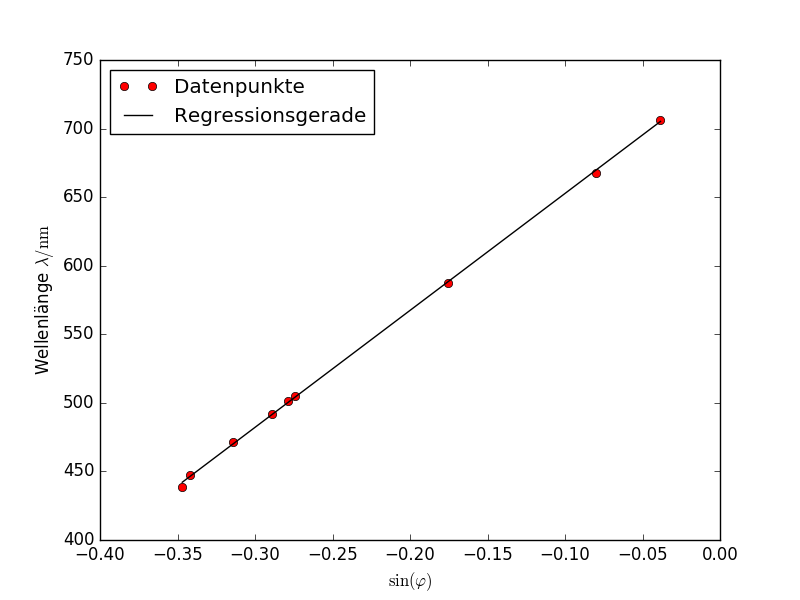
\includegraphics[width=\textwidth]{Regression.png}
	\caption{Messwerte und Regressionsgerade zur Bestimmung der Gitterkonstante}
	\label{fig:Regression}
\end{figure}
Die gemessenen Beugungswinkel aus Tabelle \ref{tab:Winkel} sind die optisch gemittelten Winkel zwischen den beiden Dublett-Linien, sodass die Funktion $\lambda(\varphi)$ auch direkt die mittlere Wellenlänge liefert. \\
\ \\
\subsection{Quantenzahlen}
Die Hauptquantenzahl $n$ und die echte Kernzahl $z$ werden einem Periodensystem entnommen. Die Bahndrehimpulszahl ist in allen Fällen $l=1$.
\clearpage
\subsection{Das Ergebnis}
Nun sind alle benötigten Größen bekannt und die Abschirmungszahl kann berechnet werden. Alle in vorigen Kapiteln besprochenen Größen, sowie die daraus resultierenden Abschirmzahlen für jedes Dublett sind je für die Elemente Natrium, Kalium und Rubidium in den Tabellen \ref{tab:Natrium}, \ref{tab:Kalium} und \ref{tab:Rubidium} dargestellt. \\

\begin{table}[h!]
    \centering
    \caption{Natrium ($n=3,z=11$) -- Abschirmungszahl für jedes betrachtete Dublett, sowie bei der Berechnung verwendete Größen}
    \label{tab:Natrium}
    \sisetup{parse-numbers=false}
    \begin{tabular}{
	S[table-format=3.0]
	@{${}\pm{}$}
	S[table-format=1.0, table-number-alignment = left]
	S[table-format=1.4]
	@{${}\pm{}$}
	S[table-format=1.4, table-number-alignment = left]
	S[table-format=2.0]
	S[table-format=1.2]
	@{${}\pm{}$}
	S[table-format=1.2, table-number-alignment = left]
	S[table-format=1.3]
	@{${}\pm{}$}
	S[table-format=1.3, table-number-alignment = left]
	}
	\toprule
	\multicolumn{2}{c}{$\lambda \ \mathrm{in} \ \si{\nano\meter}$}		& \multicolumn{2}{c}{$\Delta\lambda \ \mathrm{in} \ \si{\nano\meter}$}		& 
	{$\Delta s \ \mathrm{in} \ \mathrm{Skt}$}		& \multicolumn{2}{c}{$\Delta E_\text{D} \ \mathrm{ in } \ \si{\milli\electronvolt}$}		& 
	\multicolumn{2}{c}{$\sigma_2$}		\\ 
	\midrule
    621 & 2 & 8.93  & 0.05 & 52 & 28.7 & 0.2 & 4.20 & 0.01 \\
594 & 2 & 10.25 & 0.05 & 60 & 36.0 & 0.3 & 3.80 & 0.01 \\
572 & 2 & 6.63  & 0.03 & 39 & 25.1 & 0.2 & 4.42 & 0.01 \\

    \bottomrule
    \end{tabular}
    \end{table}

\begin{table}[h!]
    \centering
    \caption{Kalium ($n=4,z=19$) -- Abschirmungszahl für jedes betrachtete Dublett, sowie bei der Berechnung verwendete Größen}
    \label{tab:Kalium}
    \sisetup{parse-numbers=false}
    \begin{tabular}{
	S[table-format=3.0]
	@{${}\pm{}$}
	S[table-format=1.0, table-number-alignment = left]
	S[table-format=1.3]
	@{${}\pm{}$}
	S[table-format=1.3, table-number-alignment = left]
	S[table-format=3.0]
	S[table-format=1.2]
	@{${}\pm{}$}
	S[table-format=1.2, table-number-alignment = left]
	S[table-format=2.3]
	@{${}\pm{}$}
	S[table-format=1.3, table-number-alignment = left]
	}
	\toprule
	\multicolumn{2}{c}{$\lambda \ \mathrm{ in } \ \si{\nano\meter}$}		& \multicolumn{2}{c}{$\Delta\lambda \ \mathrm{ in } \ \si{\nano\meter}$}		& 
	{$\Delta s \ \mathrm{in} \ \mathrm{Skt}$}		& \multicolumn{2}{c}{$\Delta E_\text{D} \ \mathrm{ in } \ \si{\milli\electronvolt}$}		& 
	\multicolumn{2}{c}{$\sigma_2$}		\\ 
	\midrule
    587 & 2 & 22.2 & 0.1 & 130 & 79.8 & 0.6 & 18.99999273 & 0.00000001 \\
585 & 2 & 22.2 & 0.1 & 130 & 80.2 & 0.6 & 18.99999272 & 0.00000001 \\
537 & 2 & 20.0 & 0.1 & 119 & 86.0 & 0.8 & 18.99999259 & 0.00000002 \\
536 & 2 & 19.4 & 0.1 & 115 & 83.6 & 0.7 & 18.99999264 & 0.00000002 \\

    \bottomrule
    \end{tabular}
    \end{table}

\begin{table}[h!]
    \centering
    \caption{Rubidium ($n=5,z=37$) -- Abschirmungszahl für das betrachtete Dublett, sowie bei der Berechnung verwendete Größen}
    \label{tab:Rubidium}
    \sisetup{parse-numbers=false}
    \begin{tabular}{
	S[table-format=3.0]
	@{${}\pm{}$}
	S[table-format=1.0, table-number-alignment = left]
	S[table-format=1.2]
	@{${}\pm{}$}
	S[table-format=1.2, table-number-alignment = left]
	S[table-format=3.0]
	S[table-format=2.1]
	@{${}\pm{}$}
	S[table-format=1.1, table-number-alignment = left]
	S[table-format=2.2]
	@{${}\pm{}$}
	S[table-format=1.2, table-number-alignment = left]
	}
	\toprule
	\multicolumn{2}{c}{$\lambda \ \mathrm{ in } \ \si{\nano\meter}$}		& \multicolumn{2}{c}{$\Delta\lambda \ \mathrm{ in } \ \si{\nano\meter}$}		& 
	{$\Delta s \ \mathrm{in} \ \mathrm{Skt}$}		& \multicolumn{2}{c}{$\Delta E_\text{D} \ \mathrm{ in } \ \si{\milli\electronvolt}$}		& 
	\multicolumn{2}{c}{$\sigma_2$}		\\ 
	\midrule
    631 & 2 & 110.7 & 0.6 & 644 & 345 & 2 & 36.99998760 & 0.00000002 \\

    \bottomrule
    \end{tabular}
    \end{table}


Die Abschirmungszahl ist für ein Atom immer dieselbe, egal, welches Dublett betrachtet wird. Daher können die erhaltenen Werte für $\sigma_2$ gemittelt werden und  es ergeben sich die Abschrimungszahlen
\begin{align}
	\sigma_{2,\text{\ce{Na}}} &= \SI{10.999995421+-0.000000009}{}
 \\
	\sigma_{2,\text{\ce{Ka}}} &= \SI{13.12+-0.01}{}
 \\
	\sigma_{2,\text{\ce{Ru}}} &= \SI{36.99998760+-0.00000002}{}
 \ .
\end{align}